% Modified based on Xiaoming Sun's template and https://www.overleaf.com/latex/templates/cs6780-assignment-template/hgjyygbykvrf

\documentclass{scribe}
\usepackage{xfrac}
\usepackage{tikz}

\setCourse{Mathematics for Computer Science (30470023)}
\setSemester{Spring 2020}
\setInstructor{Prof. Andrew C. Yao}
\setLectureID{2}
\setLectureDate{Feb 24, 2020}
\setScribe{Boyang Chen, Jiatu Li, Mengdi Wu}
\newcommand{\prob}[1]{\mathrm{Pr} \left\{ #1 \right\}}

\begin{document}
\notetitle

\section{Overview}
\label{sec:overview}

In the second lecture, we are going to discuss three interesting and important problems as an application of discrete probability. These problems, and even solutions, are not so hard to understand for a person who rarely knows mathematics. But there is deep relationship between these problems and some mathematical theory (like coding theory), which should be considered seriously.

\section{The hat problem}
\label{sec:hats-problem}

\subsection{Problem description}
\label{sec:problem-description}

There are three people standing on the corners of a triangle, wearing hats of \textbf{black} or \textbf{\color{red}red}, which is uniformly randomly determined by the game host. They can not see the color of their own hats, but each of them can see the color of the other's. As soon as the game starts, each peron can either keep silent, or guess the color of his own hat.

The three people wins as a team if (1) at least one person takes a guess, and (2) no one guesses incorrectly. They can discuss before the game started, but after the color configuration is determined, communication of any kind is prohibited. Now they want to know that, what is their best strategy such that the probability to win is maximized.

\subsection{Strategies}
\label{sec:naive-and-clever-strategies}

Firstly we would like to discuss some naive strategies and compute their probability to win. \textit{Strategy 1} is quite simple, in which each person makes random guess. The probability for each person to be correct is $\sfrac{1}{2}$ independently, thus they win with a probability of $\left(\sfrac{1}{2}\right)^3 = \sfrac{1}{8}$. A more clever strategy, \textit{Strategy 2}, is that only one of them makes a random guess, and the other two keep silent. In this case, the probability to win is $\sfrac{1}{2}$, which is much better than \textit{Strategy 1}.

So is \textit{Strategy 2} optimal? No. The real winner is \textit{Strategy 3}, in which each person, w.l.o.g. called $A$, will look at the other two before making a decision. If the they have the same color, $A$ will choose to guess the different color and otherwise, $A$ will keep silent.

Let's consider the probability to win for \textit{Strategy 3}. If the color configuration is \textbf{BBB} or \textbf{\color{red}RRR}, each of them will make an incorrect guess and therefore they fail. Otherwise, if the color configuration is \textbf{BB{\color{red}R}}, \textbf{B{\color{red}R}B}, \textbf{B{\color{red}R}{\color{red}R}}, \textbf{{\color{red}R}BB}, \textbf{{\color{red}R}B{\color{red}R}} or \textbf{{\color{red}R}{\color{red}R}B}, only the minority will make a correct guess and they will win. As a result, the probability to win is $\sfrac{6}{8} = \sfrac{3}{4}$, which is better than $\sfrac{1}{2}$. Clever strategy! 

\subsection{Binary string and cube}
\label{sec:color-configuration}

It seems that the colorful represention will confuse us a lot when there are more than three people. Suppose $0$ denotes a \textbf{black} hat and $1$ denotes a \textbf{\color{red}red} hat, then a color configuration can be represented by a binary string of length $3$. If we draw all of the possible configurations on a three-dimensional space, we will have an unit cube (see Figure \ref{unit-cube}).

\begin{figure}[htb]
  \centering
  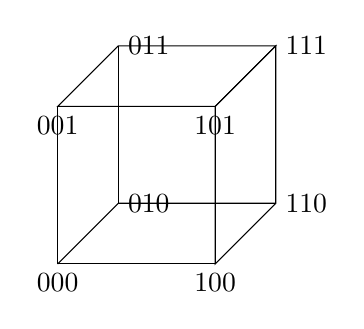
\begin{tikzpicture}
    \pgfmathsetmacro{\cubex}{2}
    \pgfmathsetmacro{\cubey}{2}
    \pgfmathsetmacro{\cubez}{2}
    \draw (-\cubex, -\cubey, 0) node[below] {$000$};
    \draw (-\cubex, 0, 0) node[below] {$001$};
    \draw (0, -\cubey, 0) node[below] {$100$};
    \draw (0, 0, 0) node[below] {$101$};
    \draw (-\cubex, -\cubey, -\cubez) node[right] {$010$};
    \draw (0, 0, -\cubez) node[right] {$111$};
    \draw (0, -\cubey, -\cubez) node[right] {$110$};
    \draw (-\cubex, 0, -\cubez) node[right] {$011$};
    \draw[] (0,0,0) -- ++(-\cubex,0,0) -- ++(0,-\cubey,0) -- ++(\cubex,0,0) -- cycle;
    \draw[] (0,0,0) -- ++(0,0,-\cubez) -- ++(0,-\cubey,0) -- ++(0,0,\cubez) -- cycle;
    \draw[] (0,0,0) -- ++(-\cubex,0,0) -- ++(0,0,-\cubez) -- ++(\cubex,0,0) -- cycle;
    \draw[] (-\cubex, -\cubey, 0) -- (-\cubex, -\cubey, -\cubez) -- (0, -\cubey, -\cubez);
    \draw[] (-\cubex, -\cubey, -\cubez) -- (-\cubex, 0, -\cubez);
  \end{tikzpicture}
  \caption{Unit-cube of all color configurations.}\label{unit-cube}
\end{figure}

Now let's look more deeper at the cube. The corners connected directly by an edge is different in exactly 1 bit. When $A$ looks at the other two, he/she can know that the actual color configuration must fall into one of the two corners $\{u, v\}$ on the cube, that are connected with an edge.
 
We would like to paint their strategy on the cube, for simplicity, let's focus on deterministic strategies. If $A$ would like to choose $u$ in $\{u, v\}$, we put an arrow from $v$ to $u$, and similarly $u\to v$ if $A$ prefers $v$. If $A$ keeps silent, we will paint nothing. For instance, Figure \ref{strategy-3} shows the cube represention of \textit{Strategy 3}.

\begin{figure}[htb]
  \centering
  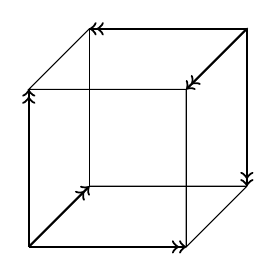
\begin{tikzpicture}
    \pgfmathsetmacro{\cubex}{2}
    \pgfmathsetmacro{\cubey}{2}
    \pgfmathsetmacro{\cubez}{2}
    \draw[] (0,0,0) -- ++(-\cubex,0,0) -- ++(0,-\cubey,0) -- ++(\cubex,0,0) -- cycle;
    \draw[] (0,0,0) -- ++(0,0,-\cubez) -- ++(0,-\cubey,0) -- ++(0,0,\cubez) -- cycle;
    \draw[] (0,0,0) -- ++(-\cubex,0,0) -- ++(0,0,-\cubez) -- ++(\cubex,0,0) -- cycle;
    \draw[] (-\cubex, -\cubey, 0) -- (-\cubex, -\cubey, -\cubez) -- (0, -\cubey, -\cubez);
    \draw[] (-\cubex, -\cubey, -\cubez) -- (-\cubex, 0, -\cubez);
    \draw[thick, ->>] (-\cubex, -\cubey, 0) -- (-\cubex, 0, 0);
    \draw[thick, ->>] (-\cubex, -\cubey, 0) -- (0, -\cubey, 0);
    \draw[thick, ->>] (-\cubex, -\cubey, 0) -- (-\cubex, -\cubey, -\cubez);
    \draw[thick, ->>] (0, 0, -\cubez) -- (0, 0, 0);
    \draw[thick, ->>] (0, 0, -\cubez) -- (0, -\cubey, -\cubez);
    \draw[thick, ->>] (0, 0, -\cubez) -- (-\cubex, 0, -\cubez);
  \end{tikzpicture}
  \caption{Cube represention of \textit{Strategy 3}.}\label{strategy-3}
\end{figure}

Intuitively speaking, \textit{Strategy 3} put the errors (source of arrows in Figure \ref{strategy-3}) into a few bad corners, so that it wins in more corners, or color configurations in the hat problem. The precious results are listed as follow.

\begin{lemma}
  \label{lemma:optimal}
  \textit{Strategy 3} is the best deterministic strategy. 
\end{lemma}
\begin{proof}
  Exercise.
\end{proof}

\begin{theorem}
  \textit{Strategy 3} is the best strategy, including those strategies with randomness.   
\end{theorem}
\begin{proof}
  Exercise.
\end{proof}

\subsection{Error correcting code}
\label{sec:ecc}

Suppose we are transmitting a binary string using a noisy channel, in which at most one bit of the string may be flipped during transmission. To ensure the correctness of transmission, we may encode $0$ into $000$ and $1$ into $111$, thus a single error can always be detected and corrected. This is a kind of \ul{1-error correcting code}.

More preciously, we choose a collection of binary string called \ul{code words} $\mathcal{C}$, such that any pair of distinct code words has disjoint neighborhood, where the neighborhood of a code word $\mathcal{N}(s)$ is defined as the set of possible strings formed by flipping a bit of $s$. In this example, we choose $\mathcal{C} = \{000, 111\}\subseteq\{0, 1\}^3$. We can transmit any binary string of length $\log_2|\mathcal{C}|$ by code words and correct any 1-bit error.

Another exmaple of the 1-error correcting code is \ul{Hamming $(7, 4)$-Code}, which choose $2^4$ code words of length $7$, thus can encode $4$-bit information. More generally, we can prove the following theorem.

\begin{theorem}
  \label{thm:hamming-exists}
  Suppose $n=2^k-1$, it's always possible to choose $2^{n-k}$ code words of length $n$ to form a 1-error correcting code, which is also optimal.   
\end{theorem}
\begin{proof}
  Firstly we prove that it's possible to choose $2^{n-k}$ code words. Suppose
  \[
    \mathcal{C} = \left\{a_1a_2\dots a_n\in \{0,1\}^n~\Big|~\bigoplus_{a_i = 1}i = 0\right\},
  \]
  is the set of code words, where $\oplus$ means bitwise xor operation. On the one hand, for all binary string $c = c_1c_2\dots c_n$, suppose $u = \oplus_{c_i=1}i$, we can find a code word
  \[c' = c_1c_2\dots c_{u-1}(1-c_u)c_{u+1}\dots c_n,\]
  such that $c\in \mathcal{N}(c')$, thus the code words and the union of their neighborhood covers all binary strings. On the other hand, it's easy to show that the neighborhoods of distinct code words are disjoint, so the code words and their neighborhoods form a partition of $\{0, 1\}^n$. Since $|\mathcal{N}(s)| = n$ for all $s$, we have
  \[ 
    |\mathcal{C}| = \frac{2^n}{|\mathcal{N}(s)| + 1} = 2^{n-k}.
  \]
  The proof of optimality is left as exercise.
\end{proof}

\subsection{The corresponding}
\label{sec:corresponding}

Now we are ready for the interesting corresponding between the hat problem and the error correcting code. The code we construct in the proof of Theorem \ref{thm:hamming-exists} is actually called \ul{perfect}, which means the code words and their neighborhood form a partition of $\{0, 1\}^n$, i.e. each binary string that is not a code word belongs to the neighborhood of some code word.

\begin{theorem}
  If there is a perfect error correcting code of length $n$, there is also an optimal strategy for the hat game of $n$ people, whose probability to win is $1-\sfrac{1}{(n+1)}$. 
\end{theorem}

\begin{proof}
  Consider the following strategy. For each person $A$, if the possible color configurations (represented by binary strings) $\{u, v\}$ in his point of view does not contain any code word, $A$ will keep silent. Otherwise w.l.o.g. $u$ is a code word, $A$ will guess that the color configuration is $v$. It's not hard to compute the probability to win and prove the optimality.  
\end{proof}

\section{Finding your IDs}

\subsection{Problem description}

$n$ students play a game. The IDs of the students are $1,2,\dots,n$, respectively. There are $n$ boxes, each of which contains one of the IDs, and no two boxes contain the same ID. During the game, each student can privately open $\frac{n}{2}$ of the boxes one by one and try to find his/her own ID. The student can discuss a strategy before the game, but no communication is allowed after the beginning of the game. If all of the students find their own IDs, they win --- then they all can avoid a final exam and get As.

\subsection{Solution}

If each student opens $\frac{n}{2}$ boxes at random, the probability of winning is only $2^{-n}$. Let's consider a more clever strategy: number the boxes from $1$ to $n$ randomly; each student first open the box with the same number as his/her ID, then repeatly open the box with the same number as the ID contained by the box he/she has just opened, until his/her ID is found or $\frac{n}{2}$ boxes has been opened.

To determine the probability of winning with this strategy, we first define a probability space $\mathbb{P} = (\mathcal{U}, p)$ by $\mathcal{U}$ being the set of ways of mapping box numbers to student IDs, i.e., the set of permutations, and $p = \frac{1}{\lvert \mathcal{U} \rvert} = \frac{1}{n!}$ since the probability is uniform.

The students win if and only if the permutation has no cycle of length over $\frac{n}{2}$. Therefore we can define the event $T$ by
\begin{align*}
  T = \left\{\sigma \mid \sigma \text{ has no cycle of length over } \frac{n}{2} \right\}.
\end{align*}
To calculate $\lvert T \rvert$, we define more events. Let $T_j$ be the set of permutations which have cycles of length $j$. Then
\begin{align*}
  \overline{T} = \bigcup_{j=\frac{n}{2}+1}^{n} T_j,
\end{align*}
and since a permutation can only have at least one cycle of length over than $\frac{n}{2}$, we have $T_j \cap T_k = \emptyset$ for all $\frac{n}{2} < j < k$. Then,
\begin{align*}
  \lvert \overline{T} \rvert = \sum_{j=\frac{n}{2}+1}^n \lvert T_j \rvert.
\end{align*}
We only need to determine $T_j$ for $j > \frac{n}{2}$. There are $\binom{n}{j}$ ways to choose the elements of the cycle. With these $j$ elements, there are $(j-1)!$ different cycles. Finally, there are $(n-j)!$ ways to arrange the rest elements. Therefore
\begin{align*}
  T_j = \binom{n}{j} (j-1)! (n-j)! = \frac{n!}{j}.
\end{align*}
The probability of winning is then given by
\begin{align*}
  \prob{T} &= 1 - \frac{\lvert \overline{T} \rvert}{\lvert \mathcal{U} \rvert} \\
           &= 1 - \sum_{i=\frac{n}{2}+1}^{n} \frac{\lvert T_j \rvert}{n!} \\
           &= 1 - \sum_{i=\frac{n}{2}+1}^{n} \frac{1}{j} \\
           &\approx 1 - (\ln n - \ln \frac{n}{2}) \\
           &= 1 - \ln 2 \\
           &\approx 30.7\%,
\end{align*}
which is surprisingly high. 

\section{The online auction problem}

\subsection{Problem description}

Here is the description of the problem: in an online auction, there are $n$ people and they will offer their bids sequentially. Suppose they offer prices randomly and none of their prices are the same (here random means that the permutation of their price is random). Then the auction goes on and we need to make a decision "to sell the goods to her" or "not to sell the goods to her" and once we reject one price we cannot accept it anymore, just as the word "online" infers. All the information we have about the price is the position of it among the $n$ prices.

The auctioneer wins if he sells the goods with the highest price among the $n$ prices. Then what is the probability he could reach to win?

We can adapt a random strategy: that is, randomly choose a number $k$ among $\{1, 2,\dots, n\}$, and accept the k-th price. We can find that the probability to win is $1/n$, which is too low to satisfy with it.

\end{document} 
